\documentclass[aps]{revtex4}
\usepackage{graphicx}
\usepackage{amssymb,amsfonts,amsmath,amsthm}
\usepackage{chemarr}
\usepackage{bm}
\usepackage{pslatex}
\usepackage{mathptmx}
\usepackage{xfrac}

%% concentration notations
\newcommand{\mymat}[1]{\boldsymbol{#1}}
\newcommand{\mytrn}[1]{{#1}^{\mathsf{T}}}
\newcommand{\myvec}[1]{\overrightarrow{#1}}
\newcommand{\mygrad}{\vec{\nabla}}
\newcommand{\myhess}{\mathcal{H}}


\begin{document}
\title{Differential Bubbles}
\maketitle

\section{Differential Properties}

\subsection{Tangent Field}
Let us assume that we have three vectors $\vec{M}_-$, $\vec{M}_0$ and $\vec{M}_+$, with
$t_-=\left\vert \myvec{M_0M_-}\right\vert$ and $t_+=\left\vert \myvec{M_0M_+}\right\vert$.
The regular curve approximation is
\begin{equation}
	\vec{M}(t) = \vec{M}_0 + t \partial_t \vec{M} + \frac{1}{2} t^2 \partial_{t}^2 \vec{M}
\end{equation}
so that
\begin{equation}
\left\lbrace
\begin{array}{rcl}
	\myvec{M_0M_-} & = & -t_- \partial_t \vec{M} + \frac{1}{2} t_-^2 \partial_{t}^2 \vec{M}\\
	\myvec{M_0M_-} & = &  t_+ \partial_t \vec{M} + \frac{1}{2} t_+^2 \partial_{t}^2 \vec{M}.\\
\end{array}
\right.
\end{equation}
Setting

\begin{equation}
\left\lbrace
\begin{array}{rcl}
	\vec{V}_- & = & \frac{1}{t_-} \myvec{M_0M_-}\\
	\vec{V}_+ & = & \frac{1}{t_+} \myvec{M_0M_+}\\
\end{array}
\right.
\end{equation}
we shall solve
\begin{equation}
	\left\lbrace
	\begin{array}{rcl}
	\vec{V}_- & = & -\partial_t \vec{M} + \frac{1}{2} t_- \partial_{t}^2 \vec{M}\\
	\vec{V}_+ & = & \partial_t \vec{M} + \frac{1}{2} t_+ \partial_{t}^2 \vec{M}.\\
	\end{array}
\right.
\end{equation}

The first order approximation of the tangent field is
\begin{equation}
	\partial_t \vec{M} =  \frac{1}{t_-+t_+} \left(t_-\vec{V}_+ - t_+ \vec{V}_-\right)
\end{equation}

\subsection{Differential properties}
Let us assume that $\vec{M}(t)$ is a local parametric estimation of a contour.
Then the tangent vector around $\vec{M}_0$ is
\begin{equation}
	\partial_t \vec{M} = 
	 \frac{1}{t_-+t_+} \left\lbrack t_-\left(\frac{1}{t_+}\myvec{M_0M_+}\right) - t_+ \left(\frac{1}{t_-}\myvec{M_0M_-}\right)\right\rbrack
\end{equation}
and the tangent vector is
\begin{equation}
	\vec{\tau} = \frac{1}{\vert \partial_t \vec{M} \vert} \partial_t \vec{M}
\end{equation}
and the normal vector is
\begin{equation}
	\vec{n} = \begin{bmatrix}
		-\tau_y\\
		\tau_x\\
	\end{bmatrix}.
\end{equation}
If $s$ were a curvilinear abscissa then we would have
\begin{equation}
	\partial_s \vec{\tau} = \kappa \vec{n}
\end{equation}
so that
\begin{equation}
	\kappa = \frac{1}{\vert\partial_t \vec{M}\vert} \vec{n}.\partial_t \vec{\tau}
\end{equation}
with
\begin{equation}
	\partial_t \vec{\tau} = \frac{1}{t_-+t_+}
	 \left\lbrack 
	 t_-\left(\frac{1}{t_+}\left(\vec{\tau}_+ - \vec{\tau}_0\right)\right) 
	- 
	t_+ \left(\frac{1}{t_-}\left(\vec{\tau}_- - \vec{\tau}_0\right)\right)
	\right\rbrack.
\end{equation}

So that the differential properties can be determined in two passes:
\begin{enumerate}
	\item Estimate $\partial_t \vec{M}$, deduce $\vec{\tau}$ and $\vec{n}$, and store $\vert\partial_t \vec{M}\vert$,
	\item then estimate $\partial_t \vec{\tau}$ and deduce $\kappa = \frac{1}{\vert\partial_t \vec{M}\vert} \vec{n}.\partial_t \vec{\tau}$.
\end{enumerate}

\section{Segmentation}
\subsection{Computing Junctions with a Grid}

To be sure that a vector between to consecutive tracers has only ONE intersection with an horizontal or a vertical
grid, we must ensure that this distance is less than $\lambda=\min(\delta x_i,\delta y_j)/2$.

\begin{center}
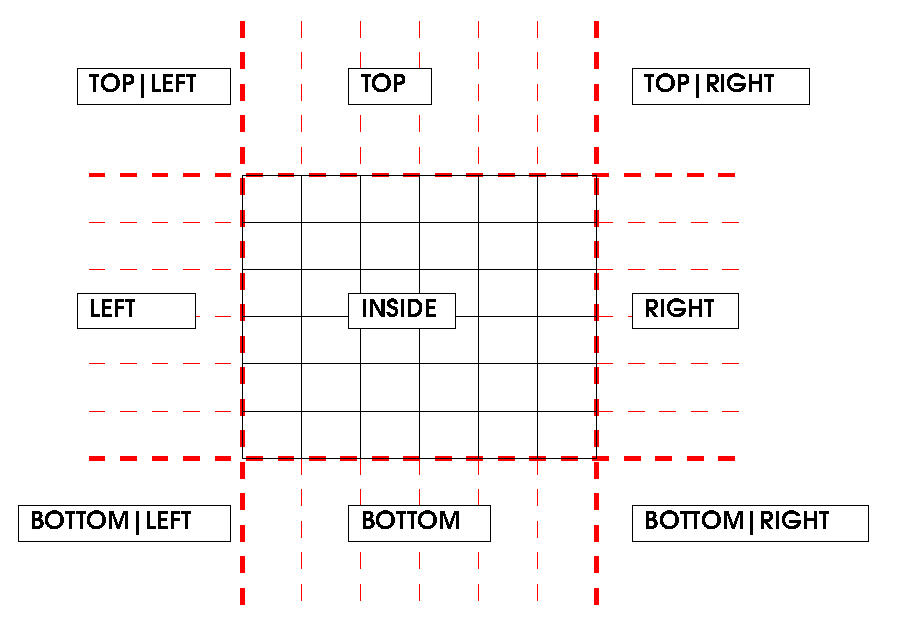
\includegraphics[scale=1]{grid.eps}
\end{center}

There is an intersection with an Horizontal axis if one of the point is Not in TOP and Not in BOTTOM and
\begin{itemize}
	\item the other point is in TOP or in BOTTOM
	\item or the other point is between two different horizontal axis (i.e. directly above or below).
\end{itemize}

There is an intersection with a Vertical axis if one of the point is Not in LEFT and Not in RIGHT and
\begin{itemize}
	\item the other point is in LEFT or in RIGHT
	\item or the other point is between to different vertical axis (i.e. directly at left or at right). 
\end{itemize}

\subsection{Segmentation by Ray Casting}
For non penetrating bubbles, the successive junctions pairs on any axis is the sequence of inside/outside positions.
When those junctions are within the grid (taking special care of sides), we mark the inner position with the owning bubble ID.

\section{Effective Pressure Field}
We need to estimate the pressure around any bulk position.
\begin{itemize}
\item
Let us assume that after the point $x_i$, there is an intersection or the bubble at $x_i + \phi$.
At this intersection, there is a pressure $P_\phi = P_{bubble} - \gamma \kappa_\phi$.
The pressure gradient can be estimated by
%$$
%	\partial_x P_j = \dfrac{1}{\phi+\delta x} 
%	\left\lbrack
%	\phi \dfrac{P_j - P_{j-1}} {\delta x} +
%	\delta x \dfrac{P_\phi - P_j}{\phi}
%	\right\rbrack = \dfrac{P_j^{L} - P_{j-1}}{2\delta_x}
%$$
$$
	\partial_x P_i = \dfrac{P_\phi - P_{i-1}}{\delta x + \phi} = \dfrac{P_i^L - P_{i-1}}{2\delta x}
$$
so that the \textit{Left Effective Pressure} is set by
$$
	P_i^L = P_{i-1} + \dfrac{2\delta x}{\phi+\delta x} \left( P_\phi - P_{i-1} \right).
$$
\item
If the intersection is at $x_i-\psi$ with $P_\psi = P_{bubble} - \gamma \kappa_\psi$
then the pressure gradient can be estimated by
$$
	\partial_x P_i = \dfrac{P_{i+1} - P_\psi}{\delta x + \psi} = \dfrac{P_{i+1}-P_i^R}{2\delta x}
$$
with the \textit{Right Effective Pressure} set by
$$
	P_i^R = P_{i+1} - \dfrac{2\delta_x}{\delta x + \psi}\left(P_{i+1} - P_\psi\right)
$$
\end{itemize}
For one dimension, we need two auxiliary pressure fields when a bulk/bubble intersection is met.

\end{document}